% This is samplepaper.tex, a sample chapter demonstrating the
% LLNCS macro package for Springer Computer Science proceedings;
% Version 2.20 of 2017/10/04
%
\documentclass[runningheads]{llncs}
%
% !TEX root = ../main.tex
%------------------------Custom Commands----------------------%

% = = = Latin Short-forms (ie, eg, etc, et al)
\usepackage{xspace}
\newcommand{\etal}{\textit{et al.}\xspace}
\newcommand{\etc}{\textit{etc.}\xspace}
\newcommand{\ie}{\textit{i.e.,}\xspace}
\newcommand{\eg}{\textit{e.g.,}\xspace}
\newcommand{\cf}{\textit{cf.}\xspace}
\newcommand{\supra}{\textit{Supra}\xspace}
\newcommand{\nee}{\textit{n\'ee}\xspace}


% = = = Arrow -> (\lt)
\newcommand{\lt}{$\rightarrow$\xspace}

% = = = Keywords (kw)
\newcommand{\kw}[1]{\textsf{#1}}

% = = = Colored text (textblue)
\newcommand{\textblue}[1]{\textcolor{blue}{#1}}

% = = = Compact Lists (compactlist, compactlistn)
\newenvironment{compactlist}
  {\begin{itemize} 
  \setlength{\itemsep}{0pt} 
  \setlength{\parskip}{0pt}} 
  {\end{itemize}}
  
\newenvironment{compactlistn}
  {\begin{enumerate} 
  \setlength{\itemsep}{0pt} 
  \setlength{\parskip}{0pt}} 
  {\end{enumerate}}
  
\renewcommand{\labelitemi}{$\bullet$}
  

%------------------------Crypto----------------------%  

% = = = Zp, Gq and Zq
\newcommand{\Zp}{\mathbb{Z}^{*}_{p}}
\newcommand{\Zq}{\mathbb{Z}_{q}}
\newcommand{\Gq}{\mathbb{G}_{q}}

% = = = Encryption, etc.
\newcommand{\Enc}[1]{\mathsf{Enc}(#1)}
\newcommand{\EncB}[1]{\llbracket #1 \rrbracket}
\newcommand{\ReRand}[1]{\mathsf{ReRand}(#1)}
\newcommand{\Hash}[1]{\mathcal{H}(#1)}
\newcommand{\Sign}[1]{\mathsf{Sig}(#1)}
\newcommand{\Comm}[1]{\mathsf{Comm}(#1)}
\newcommand{\Open}[1]{\mathsf{Open}(#1)}

% = = = Tuples
\newcommand{\tuple}[1]{\left \langle #1 \right \rangle}


%-------------------Custom for Paper----------------------%

% = = = Name
\newcommand{\ab}{\textsf{Absentia}\xspace}
\newcommand{\arb}{\textsf{Arbitrum}\xspace}





\usepackage{graphicx}
\usepackage{xcolor}
\usepackage{hyperref}
\usepackage{tikz}
% Used for displaying a sample figure. If possible, figure files should
% be included in EPS format.
%
% If you use the hyperref package, please uncomment the following line
% to display URLs in blue roman font according to Springer's eBook style:
% \renewcommand\UrlFont{\color{blue}\rmfamily}

\begin{document}
%

\title{Privacy-enhanced CBDCs}
%
%\titlerunning{Abbreviated paper title}
% If the paper title is too long for the running head, you can set
% an abbreviated paper title here
%
\author{}
%
%\authorrunning{F. Author et al.}
% First names are abbreviated in the running head.
% If there are more than two authors, 'et al.' is used.
%

%
\maketitle              % typeset the header of the contribution
%
\begin{abstract}


\keywords{}
\end{abstract}
%
%
%
\section{Related Work}
Possible CBDC designs have been extensively explored both by academics and financial institutions. Privacy is one of the significant factors that affects the design choices for CBDCs. While many works state the tradeoff between the privacy of the user and the traceability of transactions by financial regulators, a more nuanced description for a privacy model is needed by first determining the privacy requirements of each stakeholder in the system (\eg payer, payee, commercial bank, central bank). Then, the required cryptographic tools can be chosen accordingly. 


\paragraph{Transaction privacy.} Transaction privacy includes hiding the amount transacted as long as it is under a certain threshold. W{\"u}st \etal keep the transactions anonymous (payer identity, recipient, identity and the transaction value are kept hidden), as long as the transaction amount is below a certain threshold~\cite{WKCC18}. In order to determine whether the value is in a certain range, they use zero knowledge proofs. Transactions more than a determined amount should be revealed according to the rules determined by the regulatory authority. Choi \etal ~\cite{CHLRS21} and Chaum \etal ~\cite{CGM21} also discuss putting a limit for the value of transaction.

\paragraph{Information Asymmetry.} Tinn \etal utilize intentional asymmetry in their proposed CBDC design~\cite{TB21}. While the identities of the spenders cannot be associated with their purchases, the identities of the receivers are not hidden. The authority can see the identities of receiver.

Allen \etal discuss different types of privacy for a CBDC: identity privacy (the fianacial activity cannot be linked to the sender and the receiver) and transaction privacy (value, sender,and recipient of the transaction cannot be learned)~\cite{ACEF20}.

\paragraph{Token money vs account-based money.} Several works like~\cite{ACH21}, ~\cite{TB21} draw attention to the differences between account-based (similar to credit or debit card) and token money (like cash). In an account-based system, account holders are known and it is easier for regulators to analyze accounts for ensuring compliance. In a token-based systems, while users have more privacy,  as their purchases cannot be tracked, regulation becomes more difficult as purchases cannot be linked to identities. Which model is a more suitable design choice for a CBDC? Armelius \etal states that there will not be any difference between a token-based and an account-based CBDC in terms of privacy, as there is a third party (the ledger) involved~\cite{ACCH21}.

\paragraph{Transaction efficiency.} Zero-knowledge proofs help the parties validate transactions without disclosing any private information. However long generation times of these proofs creates a concern for CBDCs~\cite{ACEF20}.

\paragraph{Type of blockchain.} Some works in the literature (~\cite{WKCC18}, ~\cite{VPLP21}) explore solutions using  permissioned blockchains. Corda is used in Phase 2 of Project Jasper~\cite{CGR+17}. Corda addresses the data privacy concerns by partitioning data among the nodes, so that each node has access to only a part of data. One drawback of this approach is the challenges related to data replication across the network. These systems also introduce a point of failure at every node.

\paragraph{Privacy-preserving KYC.} Literature has also explored making regulation procedures privacy-preserving. Biryukov \etal propose a privacy-preserving KYC scheme on Ethereum, where banks can perform KYC checks using a smart contract while keeping user information hidden from other parties--only the KYC provider knows the identities~\cite{BKT18}.

\section{Conflict Diagram}
Here, we define the main stakeholders and explain the possible conflicts among them. For each conflict pair, we also define possible options to resolve the conflict between each pair. We have three main stakeholders in our diagram:

\begin{enumerate}
	\item Law enforcement: Their main aim is to prevent crime related to payments.
	\item Data holder: They are entities like commercial banks, payment processors and merchants. They want to gather, analyze and monetize the data.
	\item Privacy enthusiasts: They are typical users, regulators or privacy advocates. They want to keep their personal data private and they want to avoid intrusive and unnecessary access to their data.
	 
\end{enumerate}


\begin{figure}[htb!]
	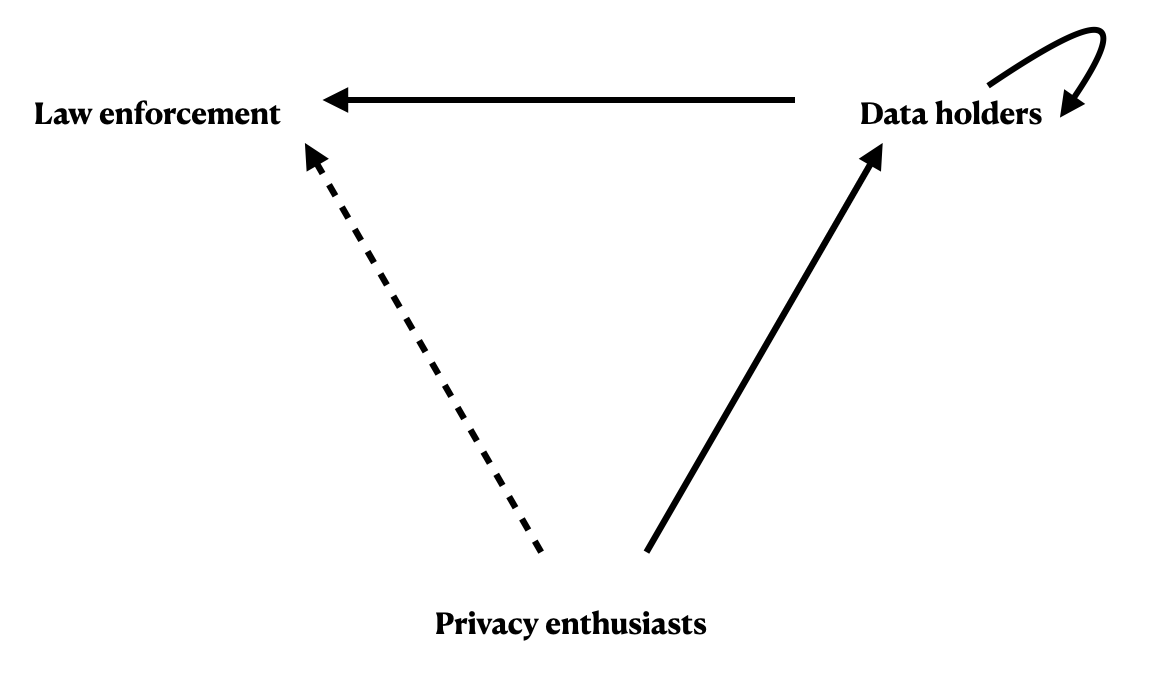
\includegraphics[width=0.7\textwidth]{figures/triangle.png}
	\caption{Conflict Diagram: The possible conflicts that can arise among law enforcement (L), data holders (D) and privacy enthusiasts (P) are captured in this conflict diagram. The conflicts are depicted as arrows between two parties. An arrow initiated from X to Y means that X has concerns about how Y operates. }
	\centering
	\label{fig:triangle}
\end{figure}

We explain each edge in Figure~\ref{fig:triangle}:
\subsection{Law enforcement - Data holders}
\paragraph{D $\rightarrow$ L:}
Data holders have concerns about the cost of maintaining their database for the law enforcement. However, they can benefit from this process if they are financially compensated.


\paragraph{L $\rightarrow$ D:} \textcolor{red}{No concern arising from the law enforcement??}

Both commercial banks and the central bank may decide to take some actions to help the law enforcement. Possible options are:
\begin{enumerate}
	\item They may not take any further action to help the law enforcement.
	\item They may follow a model which is similar to the KYC/AML scheme followed by banks today.
	\item They can choose to take action somewhere in between the previous options (\eg less stringent KYC, recording only the transactions over a certain limit). This option can be appealing especially for preventing recording too many transactions unnecessarily, as there is a cost for it.
\end{enumerate}

\subsection{Data holders - Privacy Enthusiasts}
\paragraph{D $\rightarrow$ P:} Data holders would like to monetize data. They do not want privacy to hamper their collection and analysis of data. 
\paragraph{P $\rightarrow$ D:} Privacy enthusiasts oppose indirect collection and monetization of their personal information


Possible options:
\begin{enumerate}
	\item Exceptional access: Data holders have the right to collect all data and analyze them.
	\item No access: Data collectors are not allowed to collect and analyze users data.
	\item Middle ground: Data collections is subject to a certain set of rules. Different cryptographic tools can be used to enforce these rules and define the conditions under which data collectors are allowed to see the data. Another way to enforce this is by law. 
\end{enumerate}

\subsection{Privacy Enthusiasts- Law Enforcement}
\paragraph{P $\rightarrow$ L:} Privacy enthusiasts support low crime rates but are concerned about law enforcement mistakes, corruptions and overreach.
\paragraph{L $\rightarrow$ P:} Law enforcement would like to reach data in the case of an investigation and they do not want the privacy measures to prevent them from doing so.


Possible options:
\begin{enumerate}
	\item Exceptional access: Law enforcement can reach any data any time they want.
	\item No access: Data is kept private and law enforcement cannot demand access.
	\item Middle ground: Law enforcement can access data according to certain restrictions. This can be enforced cryptographically. Another solution can be letting users to stay anonymous as long as they transact below a certain limit. All transactions above the limit are not allowed to be anonymous.
\end{enumerate}

\subsection{Data holder - Data holder}
Different data holders have conflicting interests in terms of data collection. For instance, each bank would like to be the only entity who has access to their data. This type of exclusivity is defined as \textit{horizontal exclusivity}. In contrast, consider the setting where a bank uses Visa network for credit card payments. In this case, the bank has to share its data with Visa. However, the bank is not in direct competition with the Visa network in terms of collection of the data. This type of relation is defined as \textit{vertical exclusivity}. 

In another design choice, all competitors may be obliged to share all their data with others in order to prevent monopolization of data. Using a DLT would allow every data holder to see all the data recorded, meaning that there will not be horizontal exclusivity.

Central banks want to choose what to see: they may prefer not be greedy with the data and enforce privacy, so that they will not see everything.

\newcommand{\tikzcircle}[2][black,fill=black]{\tikz[baseline=-0.5ex]\draw[#1,radius=#2] (0,0) circle ;}%

\newcommand*\halfcirc[1][1ex]{%
	\begin{tikzpicture}
	\draw[fill] (0,0)-- (90:#1) arc (90:270:#1) -- cycle ;
	\draw[thick] (0,0) circle (#1);
	\end{tikzpicture}}
% 
% \begin{table}[]
% 	
% 	\begin{tabular}{|l|c|c|c|c|c|c|}
% 		\hline
% 		&Law enf - data & \multicolumn{2}{c|}{Data  - priv} & \multicolumn{2}{c|}{Priv - Law} & Data - Data \\ \hline
% 		&               D $\rightarrow$ L      &      D $\rightarrow$ P       &   P $\rightarrow$ D            &   P $\rightarrow$ L        &     L $\rightarrow$ P       &  \\ \hline
%Cash 		         &           &           &    \tikzcircle{2pt}       &      \tikzcircle{2pt}     &           &  \\ \hline
%Visa 		           &           &  \tikzcircle{2pt}         &           &           &    \tikzcircle{2pt}       &  \\ \hline
%Bitcoin	           &           &   \halfcirc[0.5ex]         &       \halfcirc[0.5ex]    &      \halfcirc[0.5ex]    &       \halfcirc[0.5ex]       &  \\ \hline
%Zcash		          &           &           &    \tikzcircle{2pt}       &      \tikzcircle{2pt}     &           &  \\ \hline
%PRcash~\cite{WKCC18}		          &           &           &        \tikzcircle{2pt}       &       \tikzcircle{2pt}        &       \tikzcircle{2pt}        &  \\ \hline
%Privacy-preserving KYC~\cite{BKT18} 	          &            &           &           &      \tikzcircle{2pt}        &           &  \\ \hline
%Tinn \etal ~\cite{TB21}	&           &           &           &  \halfcirc[0.5ex]           &      \tikzcircle{2pt}      &            \\ \hline
%Choi \etal	~\cite{CHLRS21}	   &           &           &        \tikzcircle{2pt}       &       \tikzcircle{2pt}        &       \tikzcircle{2pt}        &  \\ \hline
%	 Chaum \etal ~\cite{CGM21}		&           &           &        \tikzcircle{2pt}       &         \tikzcircle{2pt}      &       \tikzcircle{2pt}        &            \\ \hline
%Digital Dollar~\cite{USCBDC}		&           &           &      \tikzcircle{2pt}          &     \tikzcircle{2pt}           &     \tikzcircle{2pt}           &            \\ \hline
%Fedcoin~\cite{GR16}	  &           &           &    \tikzcircle{2pt}       &      \halfcirc[0.5ex]     &    \tikzcircle{2pt}       &  \\ \hline
%CAD-Coin~\cite{GR16}				&           &           &      \tikzcircle{2pt}       &       \tikzcircle{2pt}      &     \tikzcircle{2pt}          &             \\ \hline
%e-krona~\cite{KRONA}	&           &           &       \tikzcircle{2pt}      &           &           &            \\ \hline
%%			&           &           &           &           &           &            \\ \hline
%%			&           &           &           &           &           &            \\ \hline
%
%\end{tabular}
% \end{table}

 
\section{Evaluation Framework}


\begin{table}[]
	\begin{tabular}{|l|c|c|c|c|c|}
		\hline
		&\underline{L}aw enforcement& \multicolumn{2}{c|}{\underline{P}rivacy enthusiasts} & \multicolumn{2}{c|}{\underline{D}ata holders} \\ \hline
		&    L $\rightarrow$ P   &       P $\rightarrow$ D        &      P $\rightarrow$ L        &      D $\rightarrow$ D        &     D $\rightarrow$ L          \\ \hline
		Cash 	&  &     \tikzcircle{2pt}      &    \tikzcircle{2pt}     &           &           \\ \hline
		Payment Network	& \tikzcircle{2pt} &           &           &           &           \\ \hline
		Bitcoin	&  \halfcirc[0.5ex]    &  \halfcirc[0.5ex]           &     \halfcirc[0.5ex]        &           &           \\ \hline
		Zcash	&  &   \tikzcircle{2pt}        &    \tikzcircle{2pt}       &       &           \\ \hline
		PRcash~\cite{WKCC18}		& \tikzcircle{2pt} &    ?         &   q      &           &           \\ \hline
		Privacy-preserving KYC~\cite{BKT18} 	&  &         &      \tikzcircle{2pt}        &           &           \\ \hline
%		Tinn \etal ~\cite{TB21}		&\tikzcircle{2pt}  &          &   \halfcirc[0.5ex]          &           &           \\ \hline
%		Choi \etal	~\cite{CHLRS21}		& \tikzcircle{2pt} &      \tikzcircle{2pt}      &   \tikzcircle{2pt}         &           &           \\ \hline
%		Chaum \etal ~\cite{CGM21}		&\tikzcircle{2pt}  &    \tikzcircle{2pt}        &      \tikzcircle{2pt}      &           &           \\ \hline
%		Digital Dollar~\cite{USCBDC}		& \tikzcircle{2pt}  &    \tikzcircle{2pt}        &    \tikzcircle{2pt}        &           &           \\ \hline
%		Fedcoin~\cite{GR16}	& \tikzcircle{2pt} &      \tikzcircle{2pt}     &    \halfcirc[0.5ex]        &           &           \\ \hline
%		CAD-Coin~\cite{GR16}		&\tikzcircle{2pt}  &        \tikzcircle{2pt}    &   \tikzcircle{2pt}         &           &           \\ \hline
%		e-krona~\cite{KRONA} 	& &      \tikzcircle{2pt}        &         &           &           \\ \hline
	\end{tabular}
\end{table}
 
 \subsection{Stakeholders and conflicts}
 \subsubsection{Law Enforcement}
  Their main aim is to prevent crime related to payments. 
  \paragraph{L $\rightarrow$ P}: Law enforcement would like to reach data in the case of an investigation and they do not want the privacy measures to prevent them from doing so.
  
  \begin{itemize}
  %	\item \textbf{-2:}  makes worse, how? they don’t get payment data but they get less data about something else?
  	\item \textbf{0:} L has no access to data. 
  	\item \textbf{1:} Even though L does not have full information about transactions, it can still use the data in a meaningful way for its investigations.
  	\item \textbf{2:} Privacy does not cause L any problems during investigation. The data may not be hidden and L can reach any time. Even when the data is hidden, L has the right to deanonymize it in order to use it for an investigation.
  \end{itemize}
  
  
 \subsubsection{Privacy Enthusiasts}
 They are typical users, regulators or privacy advocates. They want to keep their personal data private and they want to avoid intrusive and unnecessary access to their data.
 \paragraph{P $\rightarrow$ D:} Privacy enthusiasts oppose indirect collection and monetization of their personal information
 
   \begin{itemize}
 	\item \textbf{-2:} D can collect and analyze every data, as data is public. 
 	\item \textbf{-1:} D can learn information to a certain extent. (\eg pseudo-anonymity)
 	\item \textbf{0:} D cannot collect any data.
 	\item \textbf{1:} Certain types of data is hidden, which is enough to address P's concerns. This also does not prevent D from analyzing and collecting the data. 
 	\item \textbf{2:} 
 \end{itemize}

\paragraph{P $\rightarrow$ L:} Privacy enthusiasts support low crime rates but are concerned about law enforcement mistakes, corruptions and overreach.
   \begin{itemize}
	\item \textbf{-2:} L can collect any data.
	\item \textbf{-1:} L has privileged access to data in the case of an investigation.
	\item \textbf{0:} L has no access to data.
	\item \textbf{1:} L can access data based on a condition. For example, transactions over a certain threshold should be deanonymized and L can investigate them.
	\item \textbf{2:} 
\end{itemize}

 \subsubsection{Data Holders} 
 They are entities like commercial banks, payment processors and merchants. They want to gather, analyze and monetize the data.
 \paragraph{D $\rightarrow$ L:}
 Data holders have concerns about the cost of maintaining their database for the law enforcement. However, they can benefit from this process if they are financially compensated.
   \begin{itemize}
 	\item \textbf{-2:} D has to handle encrypted data. The cost for D to manage data is high.
 	\item \textbf{-1:} D has to maintain data. It is not encrypted, but there is still a cost for managing the records.
 	\item \textbf{0:} L does not require any collection of data.
 	\item \textbf{1:} L collects data but compensates D for it.
 	\item \textbf{2:} 
 \end{itemize}
  \paragraph{D $\rightarrow$ D:}
 Different data holders have conflicting interests in terms of data collection. For instance, each bank would like to be the only entity who has access to their data.
    \begin{itemize}
 	\item \textbf{-2:} 
 	\item \textbf{-1:} D can reach other entities' data. It creates competition.
 	\item \textbf{0:}  Data is not shared.
 	\item \textbf{1:}
 	\item \textbf{2:} 
 \end{itemize}
 
 \subsection*{Notes}
  \paragraph{Cash:}  anonymous features of cash, not traceable by L or D.
 
 \paragraph{Visa:} D and L  can trace and gather data.
 
 \paragraph{Bitcoin:}  Users remain anonymous as long as they are not associated with the address they use. D can analyze the data to a certain extent. 
 
 \paragraph{Zcash: } Similar to cash
 
 \paragraph{PRCash:} P knows that transactions are anonymous below a certain threshold. Hence, P $\rightarrow$ D and  P $\rightarrow$ L conflicts are addressed. L also knows that it can learn the details of a transactions over the threshold.
 
 \paragraph{Privacy-preserving KYC~\cite{BKT18} :} Solution to make regulation procedures privacy-preserving. P $\rightarrow$ L conflict is addressed.
 
 \paragraph{Tinn \etal ~\cite{TB21}	:} Intentional information asymmetry, identities of receivers are not hidden. The authority can see the identities of receiver. Hence partially addresses the concerns of P. 
 
 \paragraph{Choi \etal~\cite{CHLRS21}:} Similar to PRcash
 
 \paragraph{Chaum \etal~\cite{CGM21}:} Similar to PRcash
 
 \paragraph{FedCoin:} ``Fedcoin is intended as a substitute for cash and, as such, it should preserve the privacy attributes of cash (and possibly improve upon them). The primary issue is that, since the Fed acts as the gateway in and out of Fedcoin,
 it will have to know the public address of a Fedcoin recipient." As the recipient's address is not hidden  P $\rightarrow$ L conflict is addressed partially. As Fedcoin is intended as a substitute for cash, we can assume  P $\rightarrow$ D conflict is addressed
 
 \paragraph{CAD-Coin:} 
 
 ``With CAD-coin, the central bank again acts as the gateway to conversion from central bank money to CAD-coin, but privacy at conversion is not required.  The privacy requirements with CAD-coin instead relate to the needs of the non-central bank participants.  In CAD-coin, banks are still identified by a public address, but in order to complete payments requests generated from the real system, which are in terms of a bank’s legal name, a bank must know the complete list mapping of bank names to public addresses in the distributed ledger. Therefore, the only way to ensure privacy of the complete transaction record of a bank is to limit each individual bank’s access to the distributed ledger itself and to either (i) not involve all parties in transaction validation or (ii) find a way of validating the trades without seeing them, a so called “zero-knowledge validation”.~\cite{GR16}
 
 \paragraph{e-krona:} Since a permissioned ledger is used, we can assume access to data by D is controlled.
 
\section{Related work grouped according to conflict diagram}
\subsection{Law enforcement - Data Holders}
 Biryukov \etal propose a privacy-preserving KYC scheme on Ethereum, where banks can perform KYC checks using a smart contract while keeping user information hidden from other parties--only the KYC provider knows the identities~\cite{BKT18}.

\subsection{Data Holders - Privacy Enthusiasts}

\subsection{Privacy Enthusiasts - Law enforcement}
W{\"u}st \etal keep the transactions anonymous (payer identity, recipient, identity and the transaction value are kept hidden), as long as the transaction amount is below a certain threshold~\cite{WKCC18}. In order to determine whether the value is in a certain range, they use zero knowledge proofs. Transactions more than a determined amount should be revealed according to the rules determined by the regulatory authority. Choi \etal ~\cite{CHLRS21} and Chaum \etal ~\cite{CGM21} also discuss putting a limit for the value of transaction.

Tinn \etal utilize intentional asymmetry in their proposed CBDC design~\cite{TB21}. While the identities of the spenders cannot be associated with their purchases, the identities of the receivers are not hidden. The authority can see the identities of receiver.

Allen \etal discuss different types of privacy for a CBDC: identity privacy (the financial activity cannot be linked to the sender and the receiver) and transaction privacy (value, sender,and recipient of the transaction cannot be learned)~\cite{ACEF20}.

``Fedcoin is intended as a substitute for cash and, as such, it should
preserve the privacy attributes of cash (and possibly improve upon them). The primary issue is that, since the Fed acts as the gateway in and out of Fedcoin,
it will have to know the public address of a Fedcoin recipient. With CAD-coin, the central bank again acts as the gateway to conversion from central bank
money to CAD-coin, but privacy at conversion is not required.  The privacy requirements with CAD-coin instead relate to the needs of the non-central bank participants.  In CAD-coin, banks are still identified by a public address, but in order to complete
payments requests generated from the real system, which are in terms of a bank’s legal name, a bank must know the complete list mapping of bank names to public addresses in the distributed ledger. Therefore, the only way to ensure privacy of the complete transaction record of a bank is to limit each individual bank’s access to the distributed ledger itself and to either (i) not involve all parties in transaction validation or (ii) find a way of validating the trades without seeing them, a so called “zero-knowledge validation”."~\cite{GR16}

e-krona uses Corda ``For example, the e-krona’s DLT network will be private and only accessible for participants
approved by the Riksbank."~\cite{KRONA}

\subsection{Data Holder - Data Holder}
\bibliographystyle{splncs04}
\bibliography{pulp.bib}
\end{document}
